\documentclass[conference]{IEEEtran}
\IEEEoverridecommandlockouts
% The preceding line is only needed to identify funding in the first footnote. If that is unneeded, please comment it out.
\usepackage{hyperref}
\usepackage{cite}
\usepackage{amsmath,amssymb,amsfonts}
\usepackage{algorithmic}
\usepackage{graphicx}
\usepackage{textcomp}
\usepackage{xcolor}
\def\BibTeX{{\rm B\kern-.05em{\sc i\kern-.025em b}\kern-.08em
    T\kern-.1667em\lower.7ex\hbox{E}\kern-.125emX}}
\begin{document}

\title{Pixelstick\\(Version 1.0)\\
{\footnotesize}
}

\author{\IEEEauthorblockN{Oğuzhan Agkuş}
\IEEEauthorblockA{\textit{161044003} \\
\textit{agkusoguzhan@gmail.com}\\
Embedded Systems Course Final Project \\
Gebze Technical University \\
2021}
}

\maketitle

\begin{abstract}
This project implements a light painting tool for photographers. The user-friendly and flexible interface helps to shot creative photographs.
\end{abstract}

\section{Introduction}
Light painting is a term which describes photographic technique of moving a light source while taking a long exposure photograph. Using different colorful light sources in one shot creates more creative and aesthetic photographs. This technique is using in artistic and commercial projects. This project provides a useful and multi-functional tool for photographers. It uses addressable RGB LED strips as light source. This kind of LEDs on a single strip can be controlled individually thanks to chips on each LED. So, each LED can be thought as a "pixel". Since we can control the each pixel, we can draw a picture in photograph by sliding the strip horizontally. \\


\section{Review}
There is STM32 micro-controller at the center of the project. I used STM32 F411RE Nucleo board but it is not affordable for use in practice because of form factor. Although that disadvantage, it is good enough to prototyping. After all deciding all functionalities and design process a tiny PCB can be designed. I prefer WS2812B addressable RGB LED strips because they are best in price. Also their power consumption is low but they light quite bright. To provide an interface for controlling the tool, I choose Nextion touch screen. Also I need a LDR (Light Dependent Resistor) for adjusting brightness automatically. I think about adding SD card reader for make more flexible for different modes and a remote transmitter/receiver extensions for running synchronously with photograph machines. So, these extensions not available in this version of the project. \\

\subsection{Used Components}
\begin{itemize}
    \item STM32 F411RE Nucleo Board
    \item WS2812B Addressable RGB LED Strip (60 LED per meter)
    \item Nextion NX4832T035 Touch Screen
    \item LDR
\end{itemize}

\subsection{STM32 F411RE Nucleo Board}
The STM32 Nucleo board provides an affordable and flexible way for users to try out new ideas and build prototypes with any STM32 microcontroller line, choosing from the various combinations of performance, power consumption and features. The board does not require any separate probe as it integrates the ST-LINK/V2-1 debugger/programmer [1]. \\

\begin{figure}[htbp]
\centerline{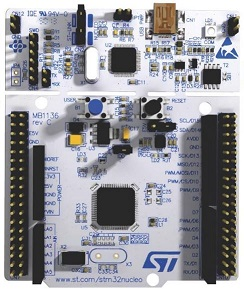
\includegraphics{stm_board.jpg}}
\caption{STM32 Nucleo Board}
\label{fig}
\end{figure}

Micro-controller features:
\begin{itemize}
    \item ARM®32-bit Cortex®-M4 CPU with FPU
    \item 100 MHz max CPU frequency
    \item 512 KB Flash
    \item 128 KB SRAM
    \item 12-bit ADC with 16 channels
    \item Timers (8)
    \item USART (3)
\end{itemize}

\subsection{WS2812B Addressable RGB LED Strip}
WS2812B is a intelligent control LED light source that the control circuit and RGB chip are integrated in a package of 5050 components. It internal include intelligent digital port data latch and signal reshaping amplification drive circuit. Also include a precision internal oscillator and a 12V voltage programmable constant current control part, effectively ensuring the pixel point light color height consistent [2]. \\ 

\begin{figure}[htbp]
\centerline{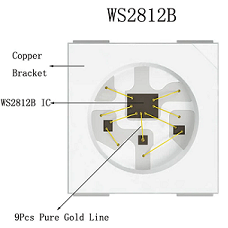
\includegraphics{ws2818b_single.png}}
\caption{WS2818 LED (single)}
\label{fig}
\end{figure}

The data transfer protocol use single NZR communication mode. After the pixel power-on reset, the DIN port receive data from controller, the first pixel collect initial 24bit data then sent to the internal data latch, the other data which reshaping by the internal signal reshaping amplification circuit sent to the next cascade pixel through the DO port. After transmission for each pixel,the signal to reduce 24bit. pixel adopt auto reshaping transmit technology, making the pixel cascade number is not limited the signal transmission, only depend on the speed of signal transmission [2]. \\

LED with low driving voltage, environmental protection and energy saving, high brightness, scattering angle is large, good consistency, low power, long life and other advantages. The control chip integrated in LED above becoming more simple circuit, small volume, convenient installation [2]. \\

\begin{figure}[htbp]
\centerline{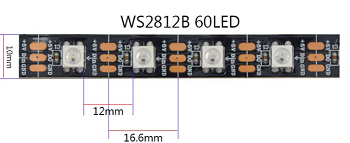
\includegraphics{ws2818b_strip.png}}
\caption{WS2818 LED (strip)}
\label{fig}
\end{figure}

\subsection{Nextion Touch Screen}
Nextion is a Human Machine Interface (HMI) solution combining an onboard processor and memory touch display with Nextion Editor software for HMI GUI project development [3]. \\

Using the Nextion Editor software, you can quickly develop the HMI GUI by drag-and-drop components (graphics, text, button, slider etc.) and ASCII text based instructions for coding how components interact at display side [3]. \\

Nextion HMI display connects to peripheral MCU via TTL Serial (5V, TX, RX ,GND) to provide event notifications that peripheral MCU can act on, the peripheral MCU can easily update progress and status back to Nextion display utilizing simple ASCII text based instructions [3]. \\

\begin{figure}[htbp]
\centerline{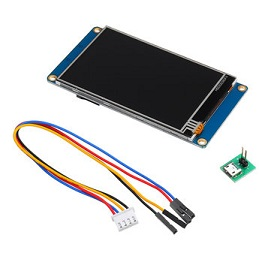
\includegraphics{nextion.jpg}}
\caption{Nextion Touch Screen}
\label{fig}
\end{figure}

\subsection{LDR}
A photoresistor (also known as a light-dependent resistor, LDR, or photo-conductive cell) is a passive component that decreases resistance with respect to receiving luminosity (light) on the component's sensitive surface. The resistance of a photoresistor decreases with increase in incident light intensity; in other words, it exhibits photoconductivity. A photoresistor can be applied in light-sensitive detector circuits and light-activated and dark-activated switching circuits acting as a resistance semiconductor [3]. \\

\section{Detail}

\subsection{Touch Screen Interface}
Nextion gives us a designer for screens. I use it to design my interfaces. In this version of the project there are 3 screens. It communicates with the micro-controller using UART. At opening and resetting it receives reset commands for all variables. During execution, it transmits 6-byte long commands to controller. Controller catch and execute coming commands.

\subsubsection{Opening Screen}
User will see these screen at opening and every reset. Brightness is 127 as default. 127 means half of the brightness. Since RGB values are 8-bit, 127 is half of 255. Brightness can be controlled by touching the slider. When auto brightness is activated, brightness data will read from LDR and brightness will set automatically. If there is more ambient light, it means LEDs will light brighter. Because our purpose is not lightning the ambiance, it is make LEDs more visible in the photograph. The brightness value sent to controller in each change. \\

\begin{figure}[htbp]
\centerline{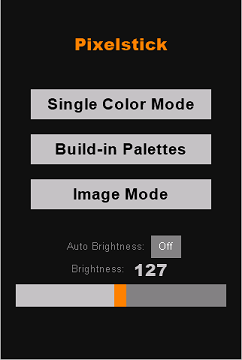
\includegraphics{opening.png}}
\caption{Opening Screen}
\label{fig}
\end{figure}

There are there 3 buttons in this screen. "Single Color Mode" and "Build-in Palettes" buttons redirects to related page. Image mode will start to light a sample image which is hard-coded. It reads pixel-values from a regular array. But it is not feasible. After adding a SD cart reader, it will read from SD card according to selected image. This feature will be available on upcoming versions of the project. Also I'm planning to add animations for LED's \\

\subsubsection{Single Color Mode}
You can set a single color for whole strip. Red, green and blue values are adjustable. The LED's 24-bit color (8-bit each main color), so values should be between 0-255. After choosing values, you must press to "Apply" button to update the strip. "Back" button returns to opening screen.

\begin{figure}[htbp]
\centerline{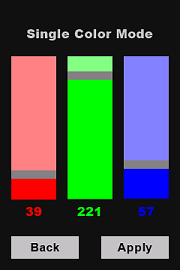
\includegraphics{single_color.png}}
\caption{Single Color Mode}
\label{fig}
\end{figure}

\subsubsection{Build-in Palettes}
In this screen you can choose 4 different built-in palettes. Pressing a button immediately apply the pixels.

\begin{figure}[htbp]
\centerline{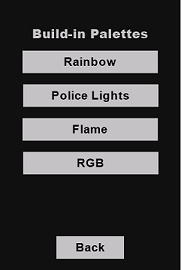
\includegraphics{palettes.png}}
\caption{Build-in Palettes}
\label{fig}
\end{figure}

\newpage

\subsection{Driving Addressable LEDs}
The LED's are driven with PWM signals. After updating pixel values memory, it is written to directly timer which generates PWM via DMA. It is very useful because it does not block execution of main loop.

\subsection{Auto Brightness}
This process is conversion from analog to digital. It performs 8-bit conversion which is good for us. The conversion is only done if auto brightness is "on". It does not waste clock cycles and consume energy.

\section{Result and Conclusion}
This version is good starting to build a perfect tool. But this version is not completely perfect. SD card extension will be so useful. Also after completing all featueres, it requires a case for use in field. \\

There some example shots taken with this tool.

\begin{figure}[htbp]
\centerline{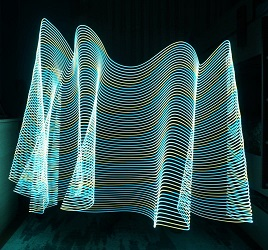
\includegraphics{1.jpg}}
\label{fig}
\end{figure}

\begin{figure}[htbp]
\centerline{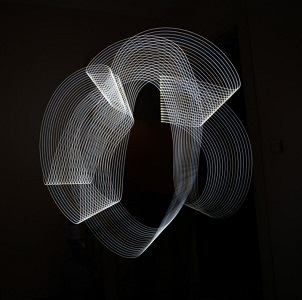
\includegraphics{2.jpg}}
\label{fig}
\end{figure}

\begin{figure}[htbp]
\centerline{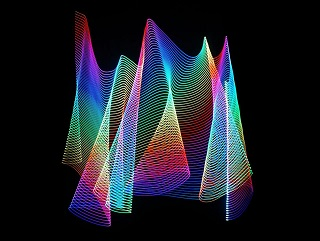
\includegraphics{3.jpg}}
\label{fig}
\end{figure}

\newpage


\section{References}
\\
1- STM32 Official Web Site\\
2- WS2812B Datasheet\\
3- Nextion Official Web Site\\

\end{document}
